\chapter{Resultados Preliminares}\label{cap_resultados}

Nesse capítulo são exibidos os resultados de alguns testes em funções reais em $\R^2$. Em cada teste, 
8 populações com 1000 indivíduos com cromossomos de 32 bits são evoluídas por 100 gerações. O espaço de busca
considerado foi $ [-1,1] \times [-1, 1] $, onde os indivíduos foram distribuídos aleatoriamente. 
O valor usado para o parâmetro da função desempenho foi $h = 2$,
as configurações para a elite foram $e_1 = 4$, $e_2 = 6$ e $e_3 = 10$ e as probabilidades de mutação $p_2$ e $p_3$ escolhidas
foram $p_2 = 5\%$ e $p_3 = 5\%$.

Ao final do processo,
foram gerados gráficos com as curvas de nível de cada função e com as posições de todos os
integrantes de todas as populações. Os 8 melhores indivíduos são marcados de forma distinta,
afim de atestar se o algoritmo foi capaz ou não de encontrar a solução real do problema.
Um segundo gráfico com os valores das funções dos 200 melhores indivíduos de cada população
no decorrer das gerações foi gerado, a fim de mostrar, em caso de convergência, sua rapidez.

Ambos os gráficos foram feitos novamente com probabilidades de mutação $p_2 = p_3 = 20\%$
para demonstrar o papel da mutação no decorrer do algoritmo, e averiguar seu impacto na diversidade genética
dos indivíduos.
Por fim, é feita uma breve discussão sobre a performance da implementação do algoritmo e sua
complexidade de tempo de execução.

\section{Testes em Funções}

\subsection{Cosseno Amortecido}

\begin{figure}
  \begin{subfigure}{\textwidth}
    \centering
    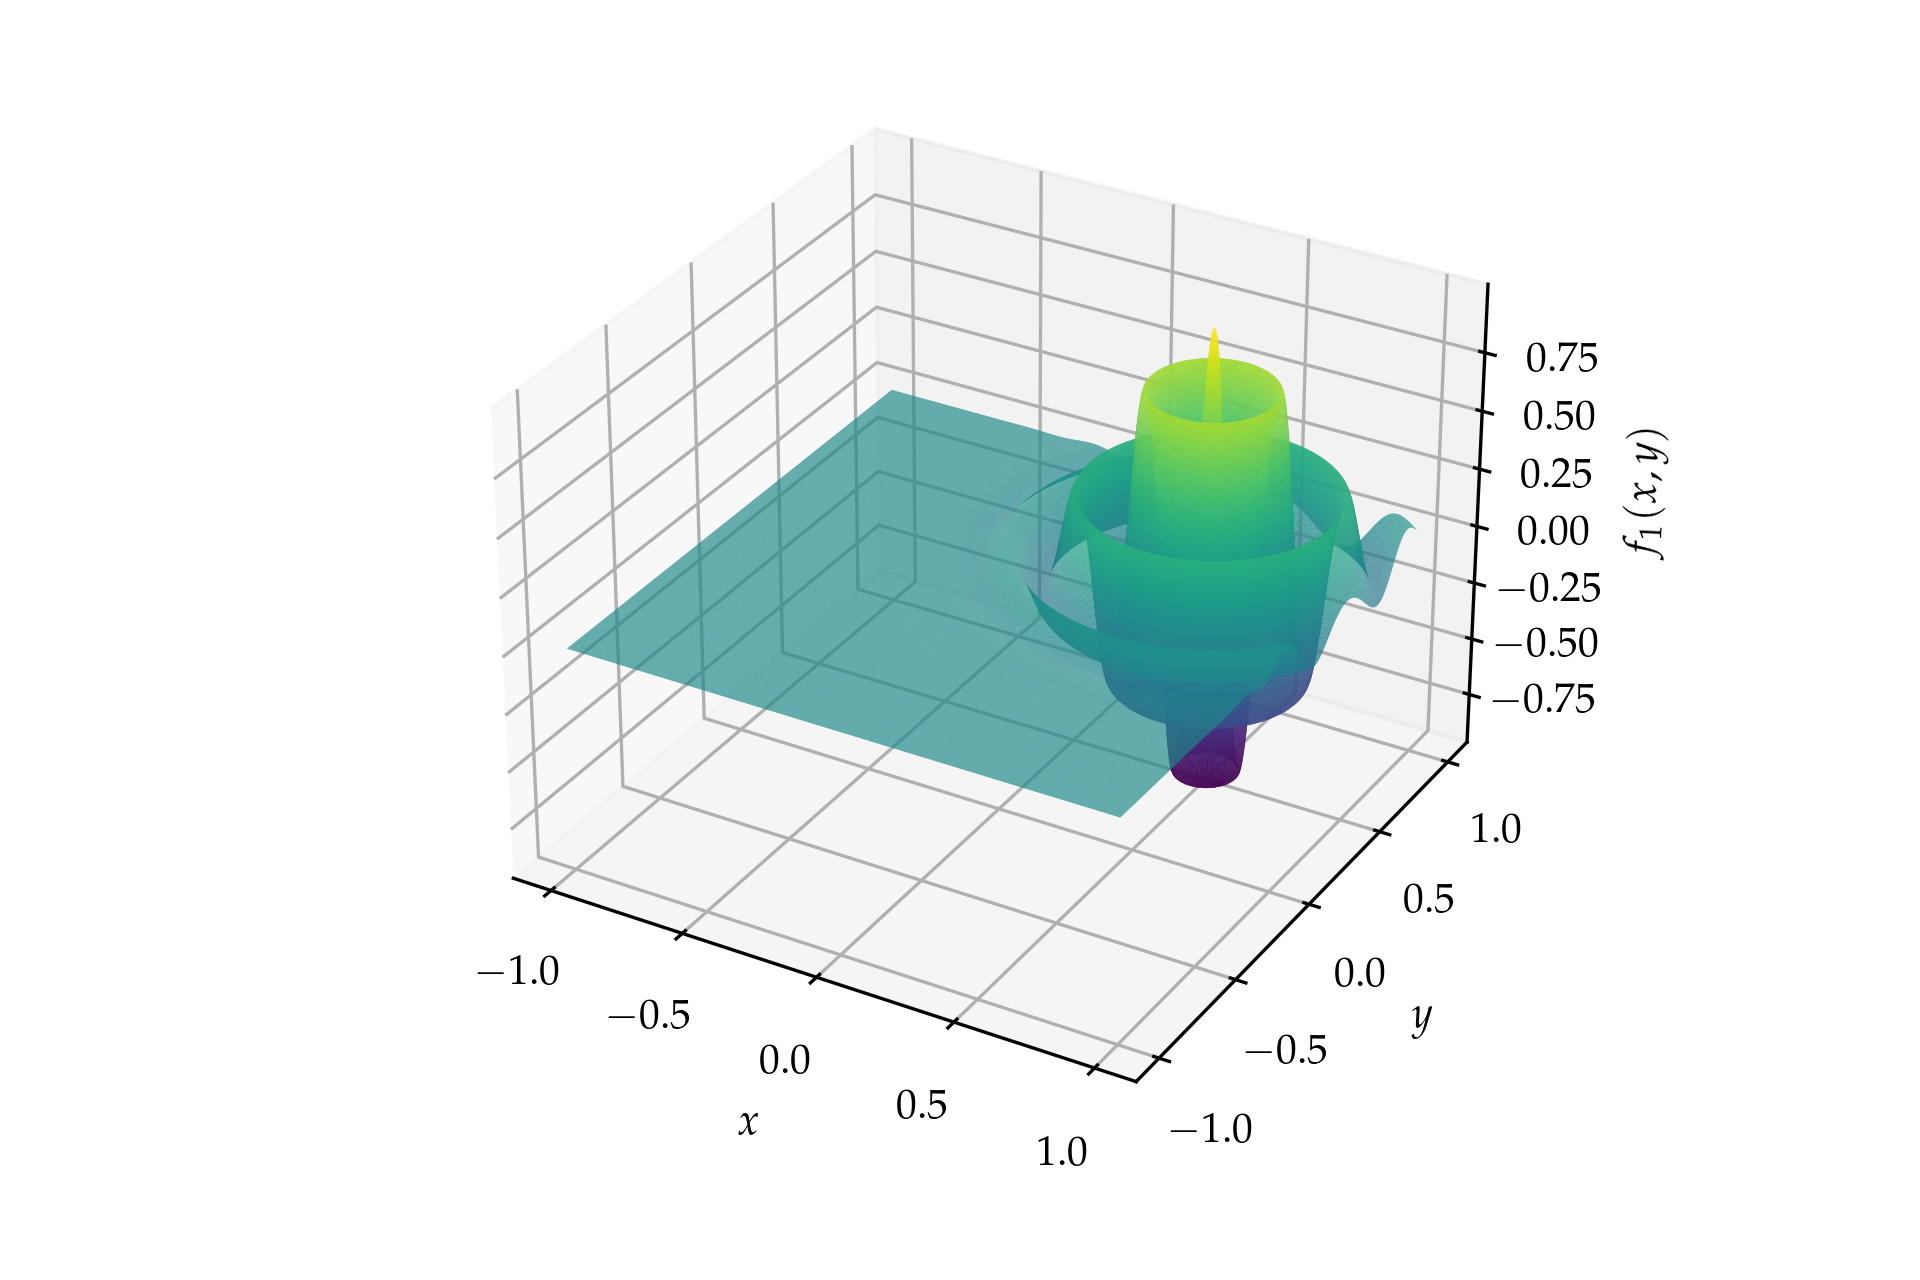
\includegraphics[width=\textwidth]{imagens/graph_damped_cossine.png}
    \caption{}
    \label{fig:graph_damped_cossine}
  \end{subfigure}
  \begin{subfigure}{\textwidth}
    \centering
    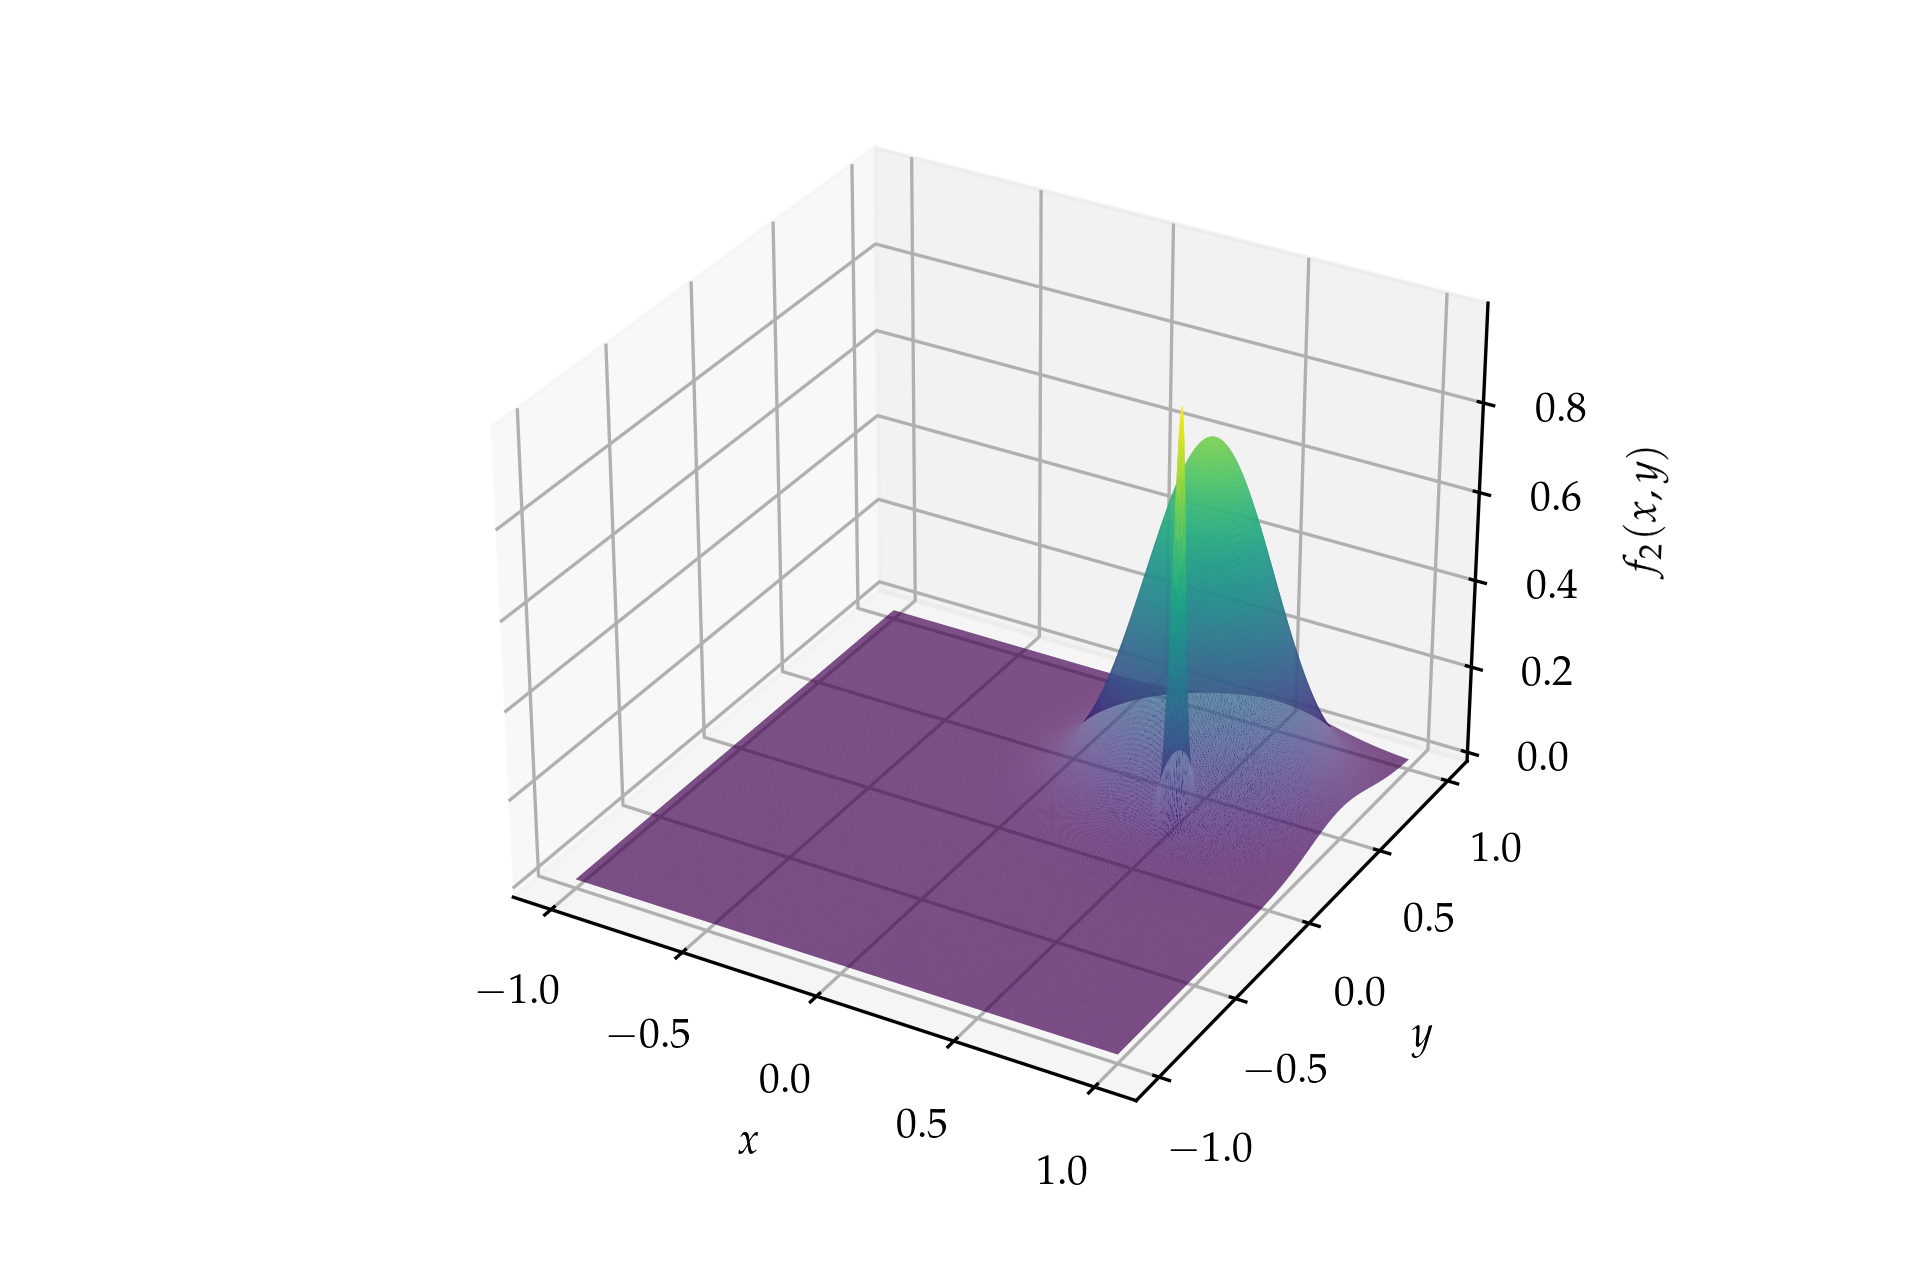
\includegraphics[width=\textwidth]{imagens/graph_near_gaussians.png}
    \caption{}
    \label{fig:graph_near_gaussians}
  \end{subfigure}
  \caption{
    \subref{fig:graph_damped_cossine} Gráfico da função $f_1(x,y)$.
    \subref{fig:graph_near_gaussians} Gráfico da função $f_2(x,y)$.
  }
\end{figure}

A primeira função testada foi
\begin{align}
  \begin{split}    
    f_1(x,y) & = \cos(9\pi r)\exp\left\{-\frac{r^2}{(0,4)^2}\right\} \;\text{, com} \\
    r      & = \sqrt{
      \left(x - 0,5\right)^2 +
      \left(y - 0,5\right)^2
    }
  \end{split}
  \label{eq:func_damped_cossine}
\end{align}
e os resultados obtidos estão dispostos nas Figuras \ref{fig:contour_damped_cossine},
\ref{fig:evolution_damped_cossine}, \ref{fig:contour_damped_cossine_mut_20} e 
\ref{fig:evolution_damped_cossine_mut_20}.

\subsection{Gaussianas Próximas}

A segunda função testada foi
\begin{align}
  \begin{split}
    f_2(x,y) & = 0,8 \exp\left\{-\frac{r_1^2}{(0,3)^2}\right\} +
    0,88 \exp\left\{-\frac{r_2^2}{(0,03)^2}\right\} \;\text{, onde} \\
    r_1      & = \sqrt{
      \left(x - 0,5\right)^2 +
      \left(y - 0,5\right)^2
    } \;\text{ e} \\
    r_2      & = \sqrt{
      \left(x - 0,6\right)^2 +
      \left(y - 0,1\right)^2
    } \mathcomma
  \end{split}
  \label{eq:func_near_gaussians}
\end{align}
com os resultados obtidos ilustrados nas Figuras \ref{fig:contour_near_gaussians},
\ref{fig:evolution_near_gaussians}, \ref{fig:contour_near_gaussians_mut_20} e 
\ref{fig:evolution_near_gaussians_mut_20}.

\begin{figure}[p]
  \centering
  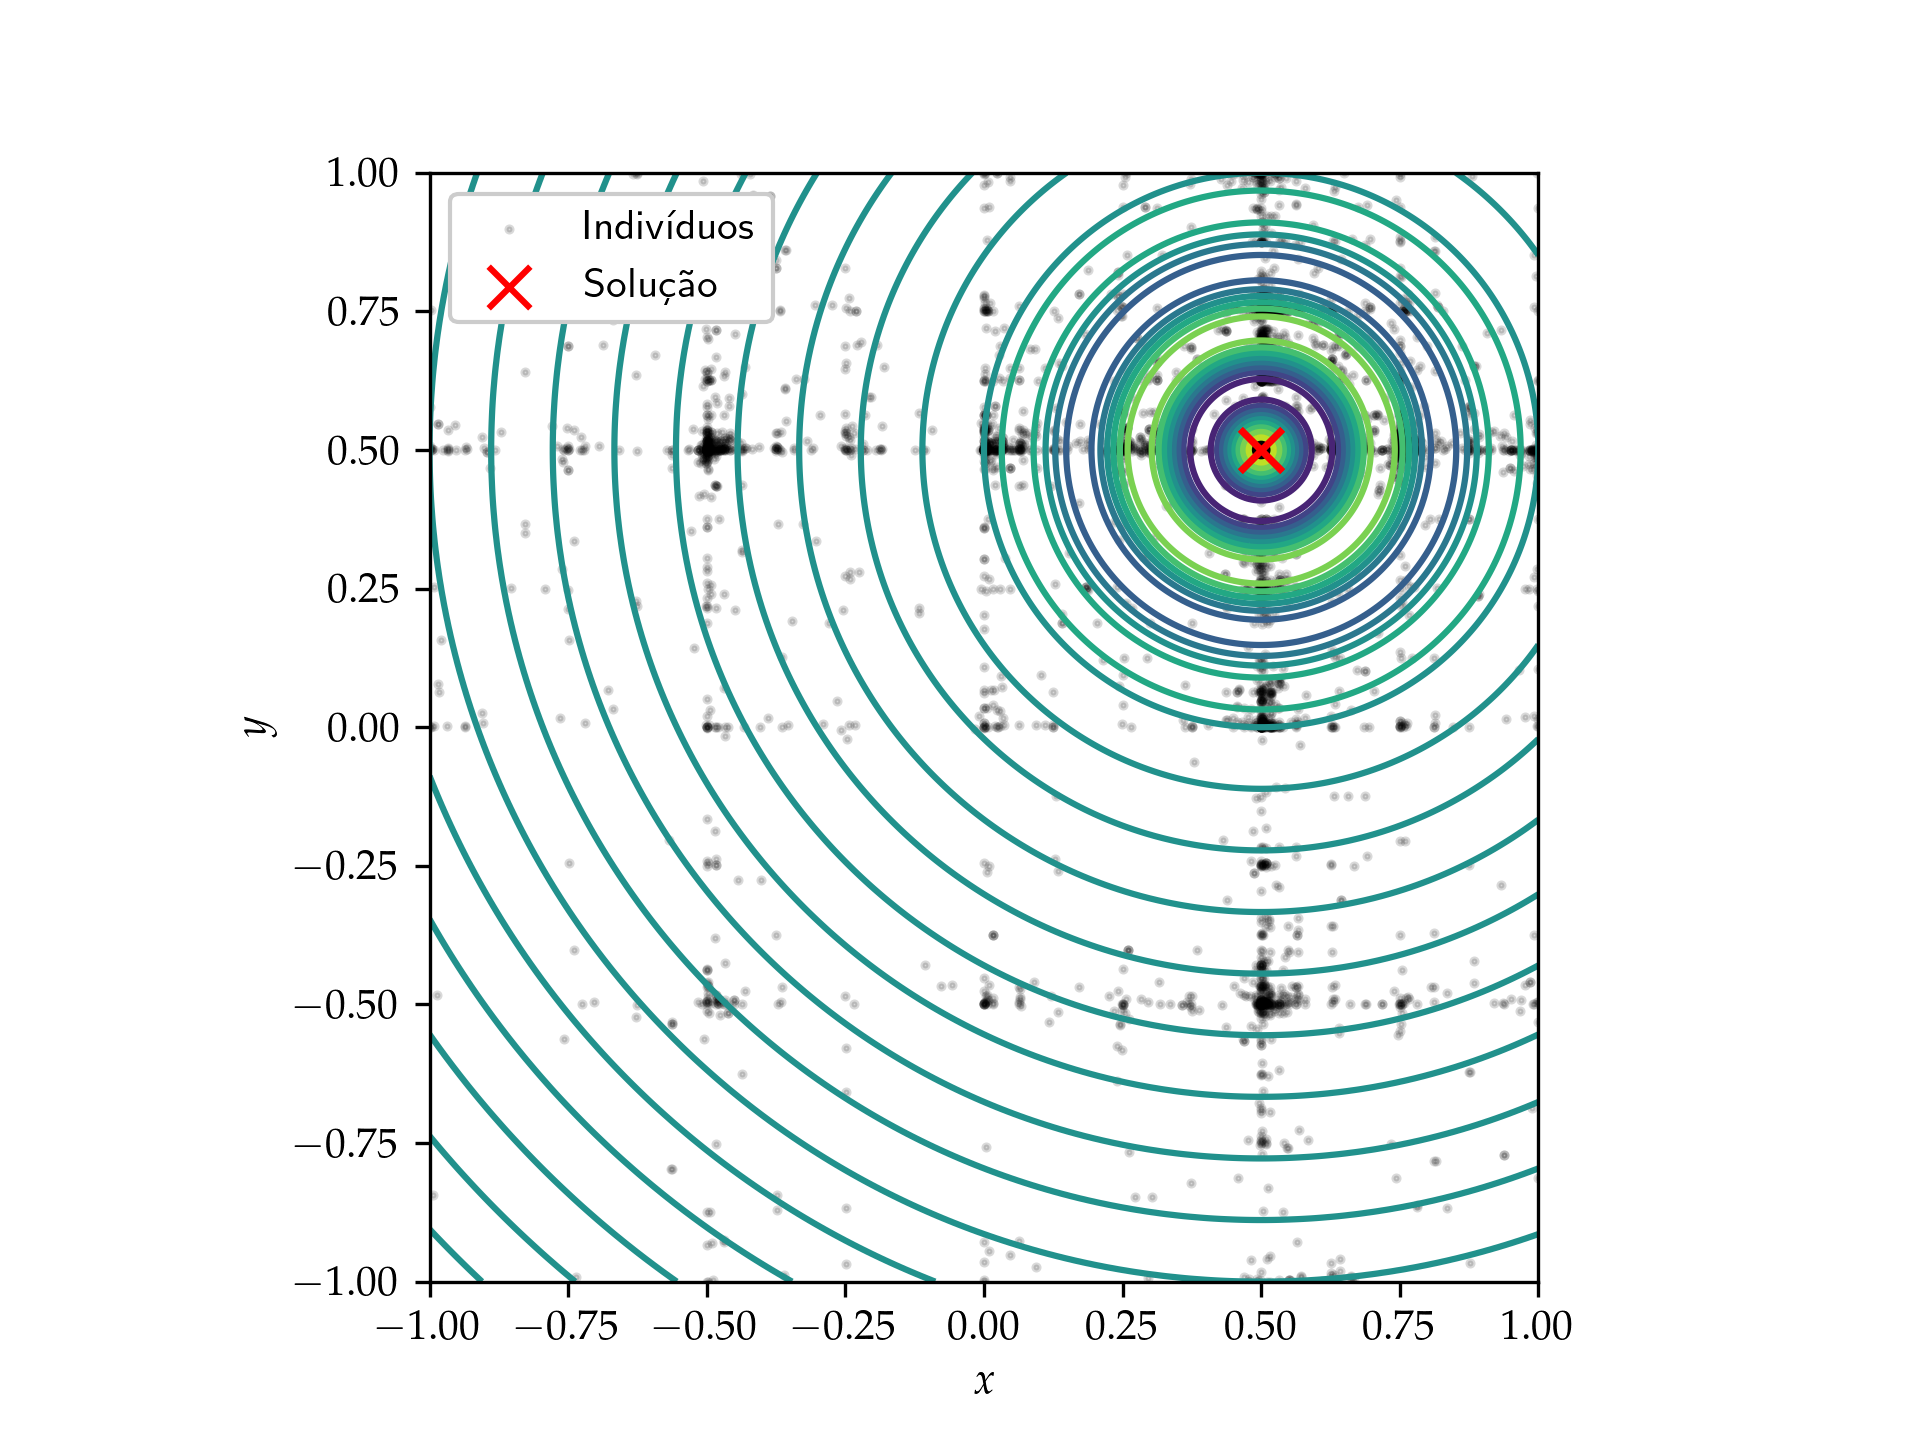
\includegraphics[width=\textwidth]{imagens/low_prob/contour_damped_cossine.png}
  \caption{
    Curvas de nível da função $f_1(x,y)$. Os pontos em preto indicam as posições dos indivíduos
    de 8 populações em sua 100ª geração na otimização da função, com $ p_2 = p_3 = 5\% $. 
    Marcado com um $\times$ vermelho estão os melhores indivíduos de cada população.
  }
  \label{fig:contour_damped_cossine}
\end{figure}

\begin{figure}[p]
  \centering
  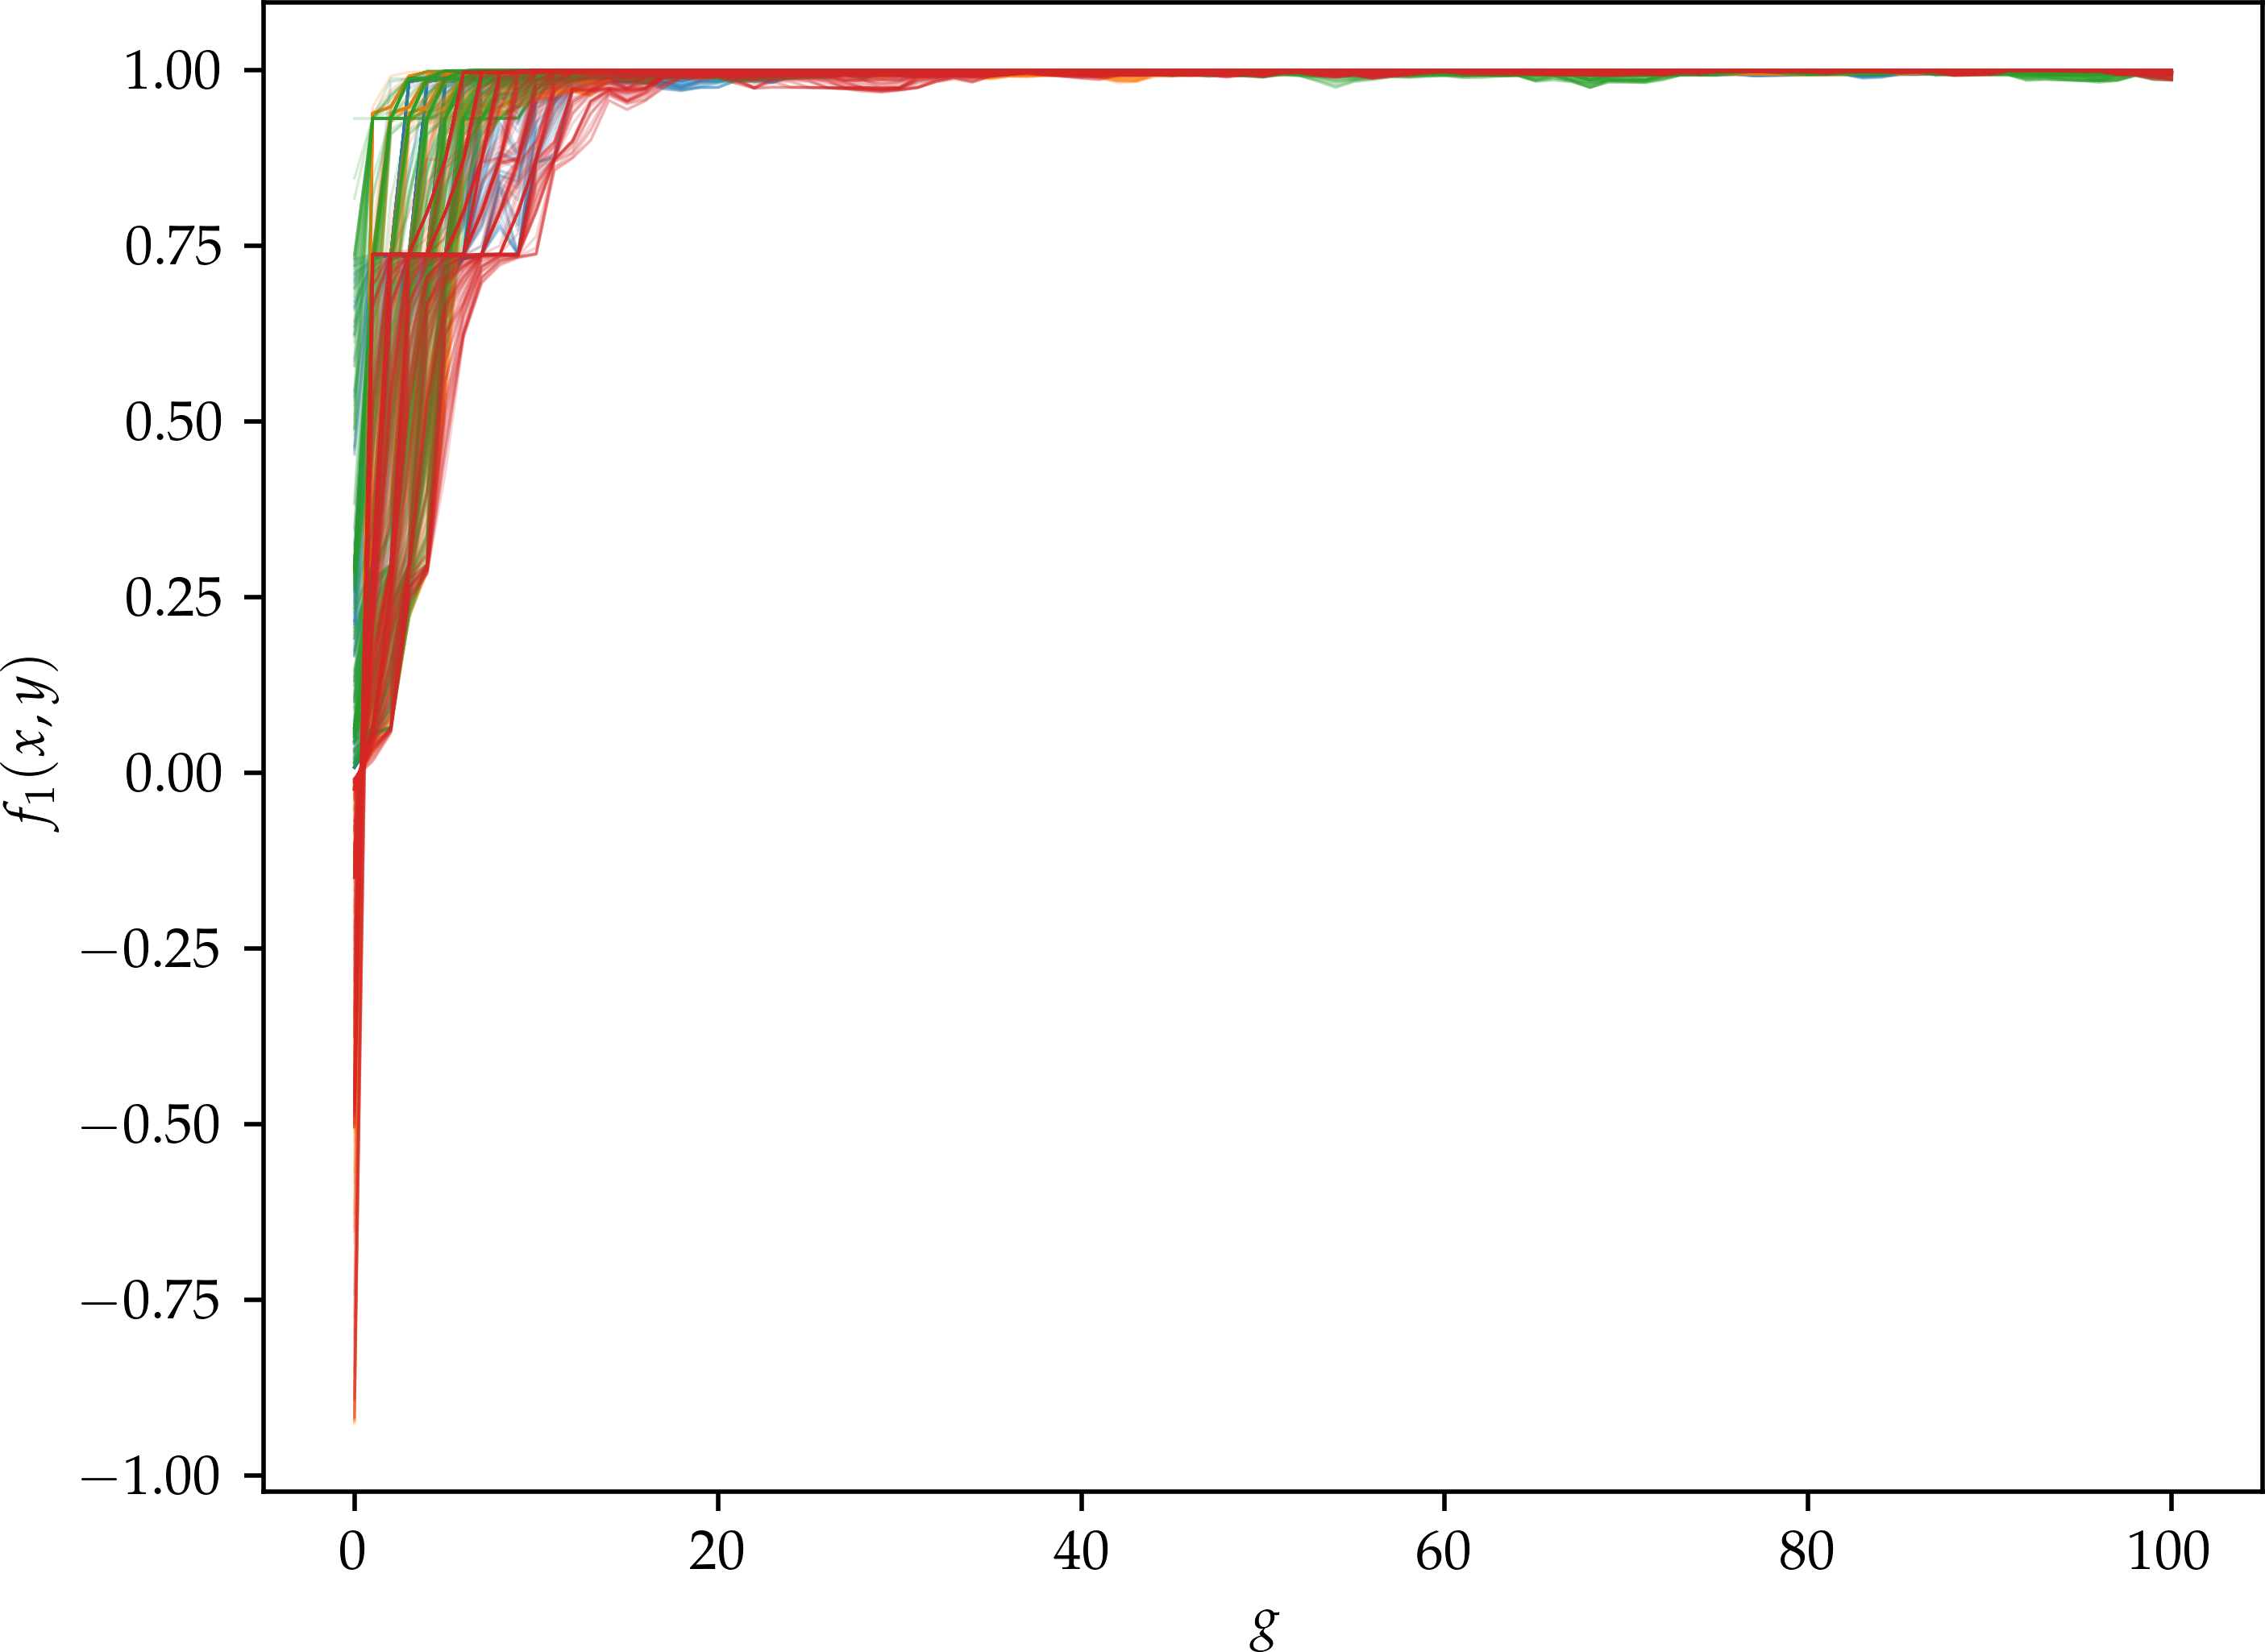
\includegraphics[width=\textwidth]{imagens/low_prob/evolution_damped_cossine.png}
  \caption{
    Evolução dos valores da função $ f_1(x,y) $ para os
    melhores 200 indivíduos de cada população, diferenciadas por cor, em termos da geração $g$,
    com $ p_2 = p_3 = 5\% $.
  }
  \label{fig:evolution_damped_cossine}
\end{figure}

\begin{figure}[p]
  \centering
  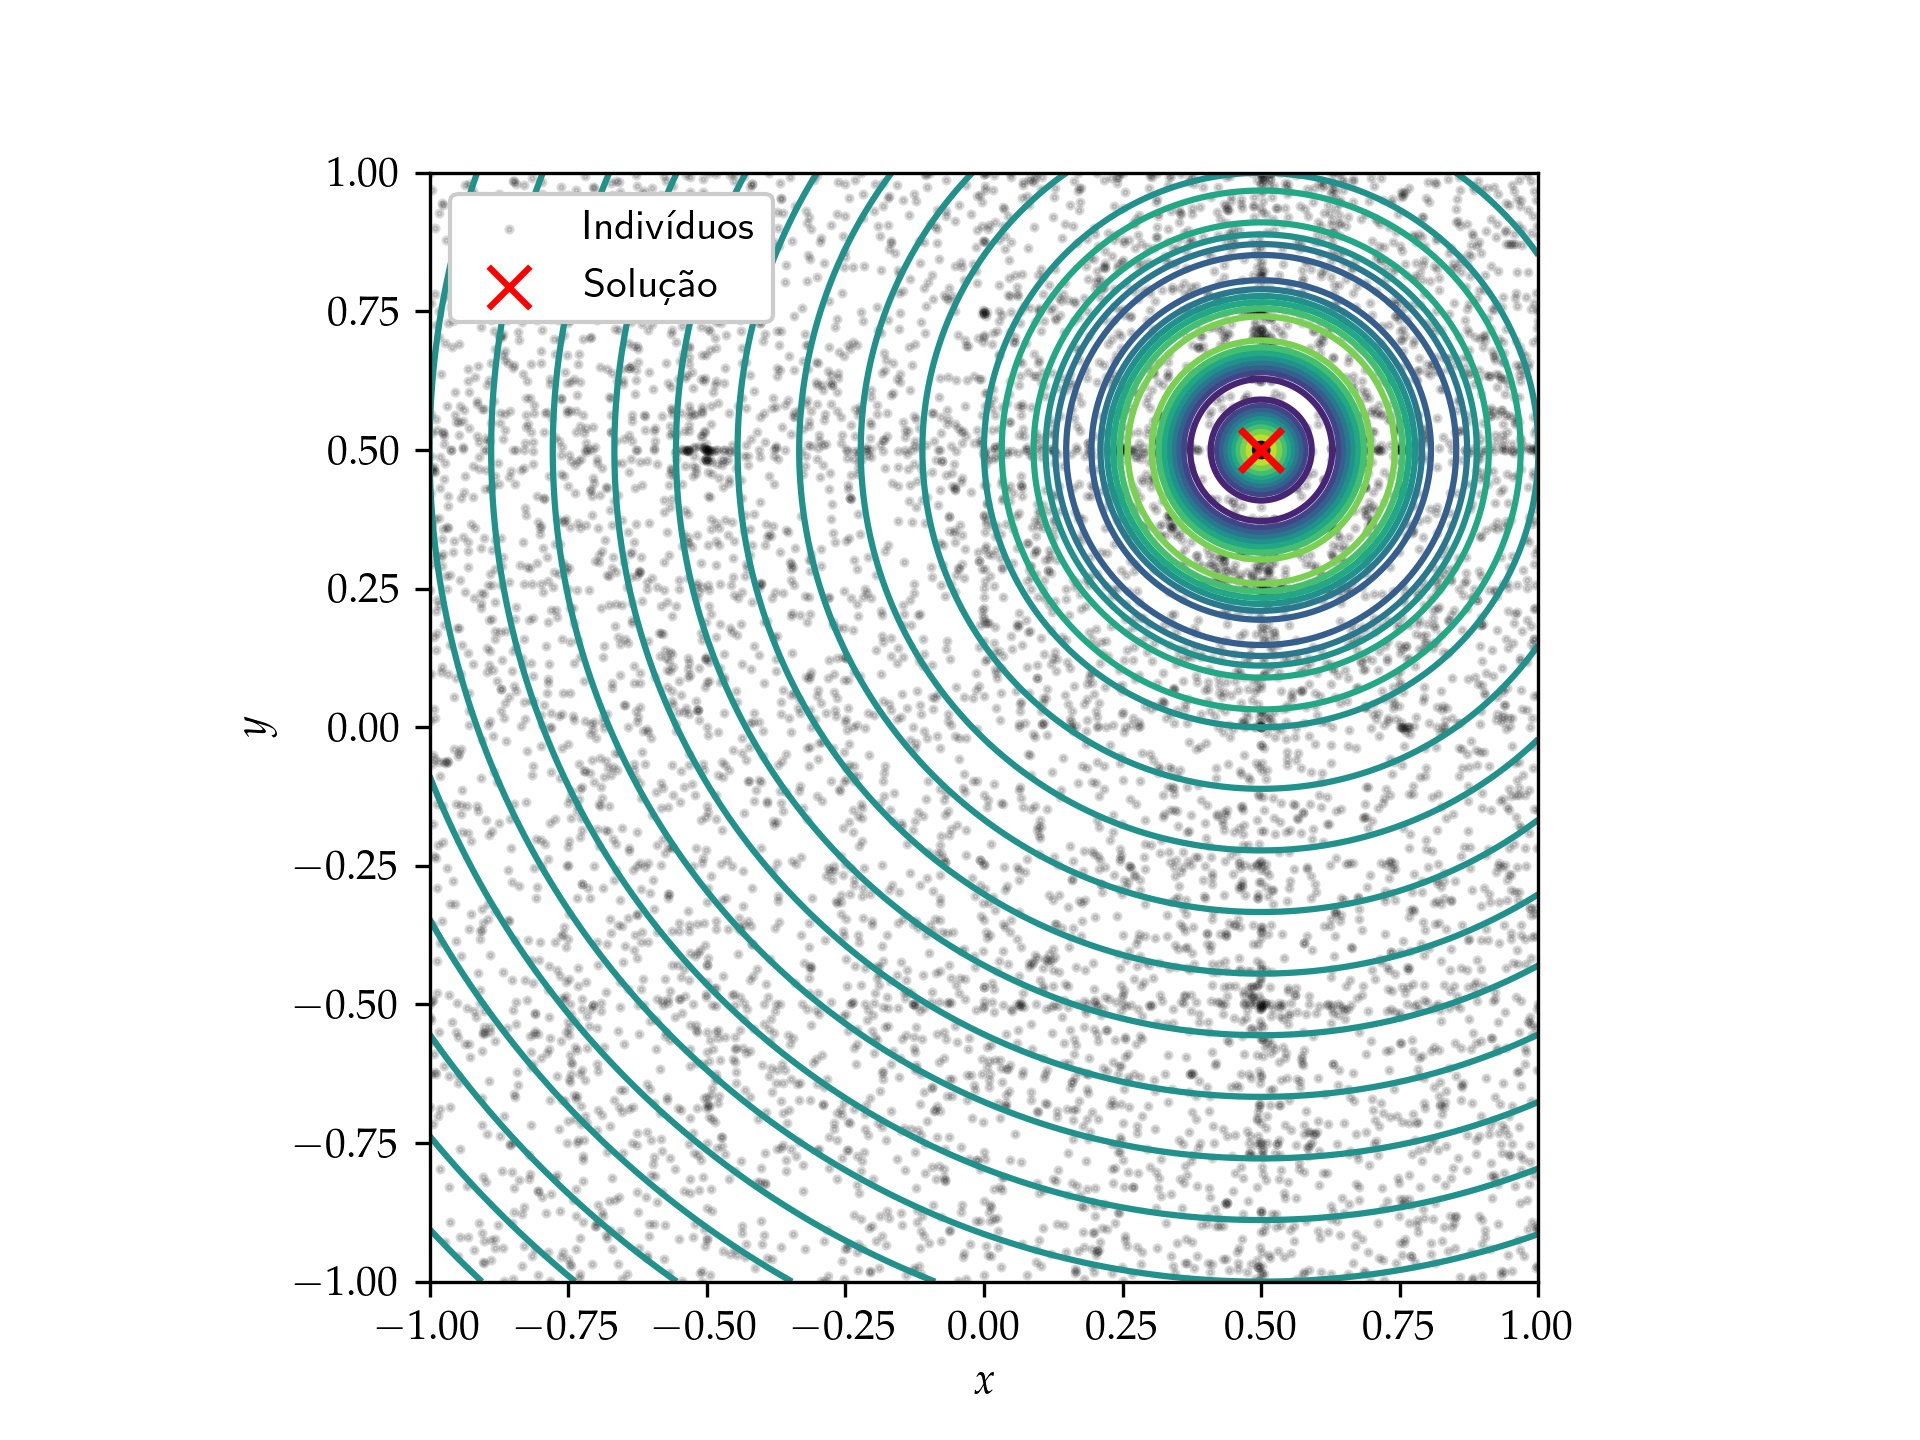
\includegraphics[width=\textwidth]{imagens/high_prob/contour_damped_cossine.png}
  \caption{
    Curvas de nível da função $f_1(x,y)$. Os pontos em preto indicam as posições dos indivíduos
    de 8 populações em sua 100ª geração na otimização da função, com $ p_2 = p_3 = 20\% $. 
    Marcado com um $\times$ vermelho estão os melhores indivíduos de cada população.
  }
  \label{fig:contour_damped_cossine_mut_20}
\end{figure}

\begin{figure}[p]
  \centering
  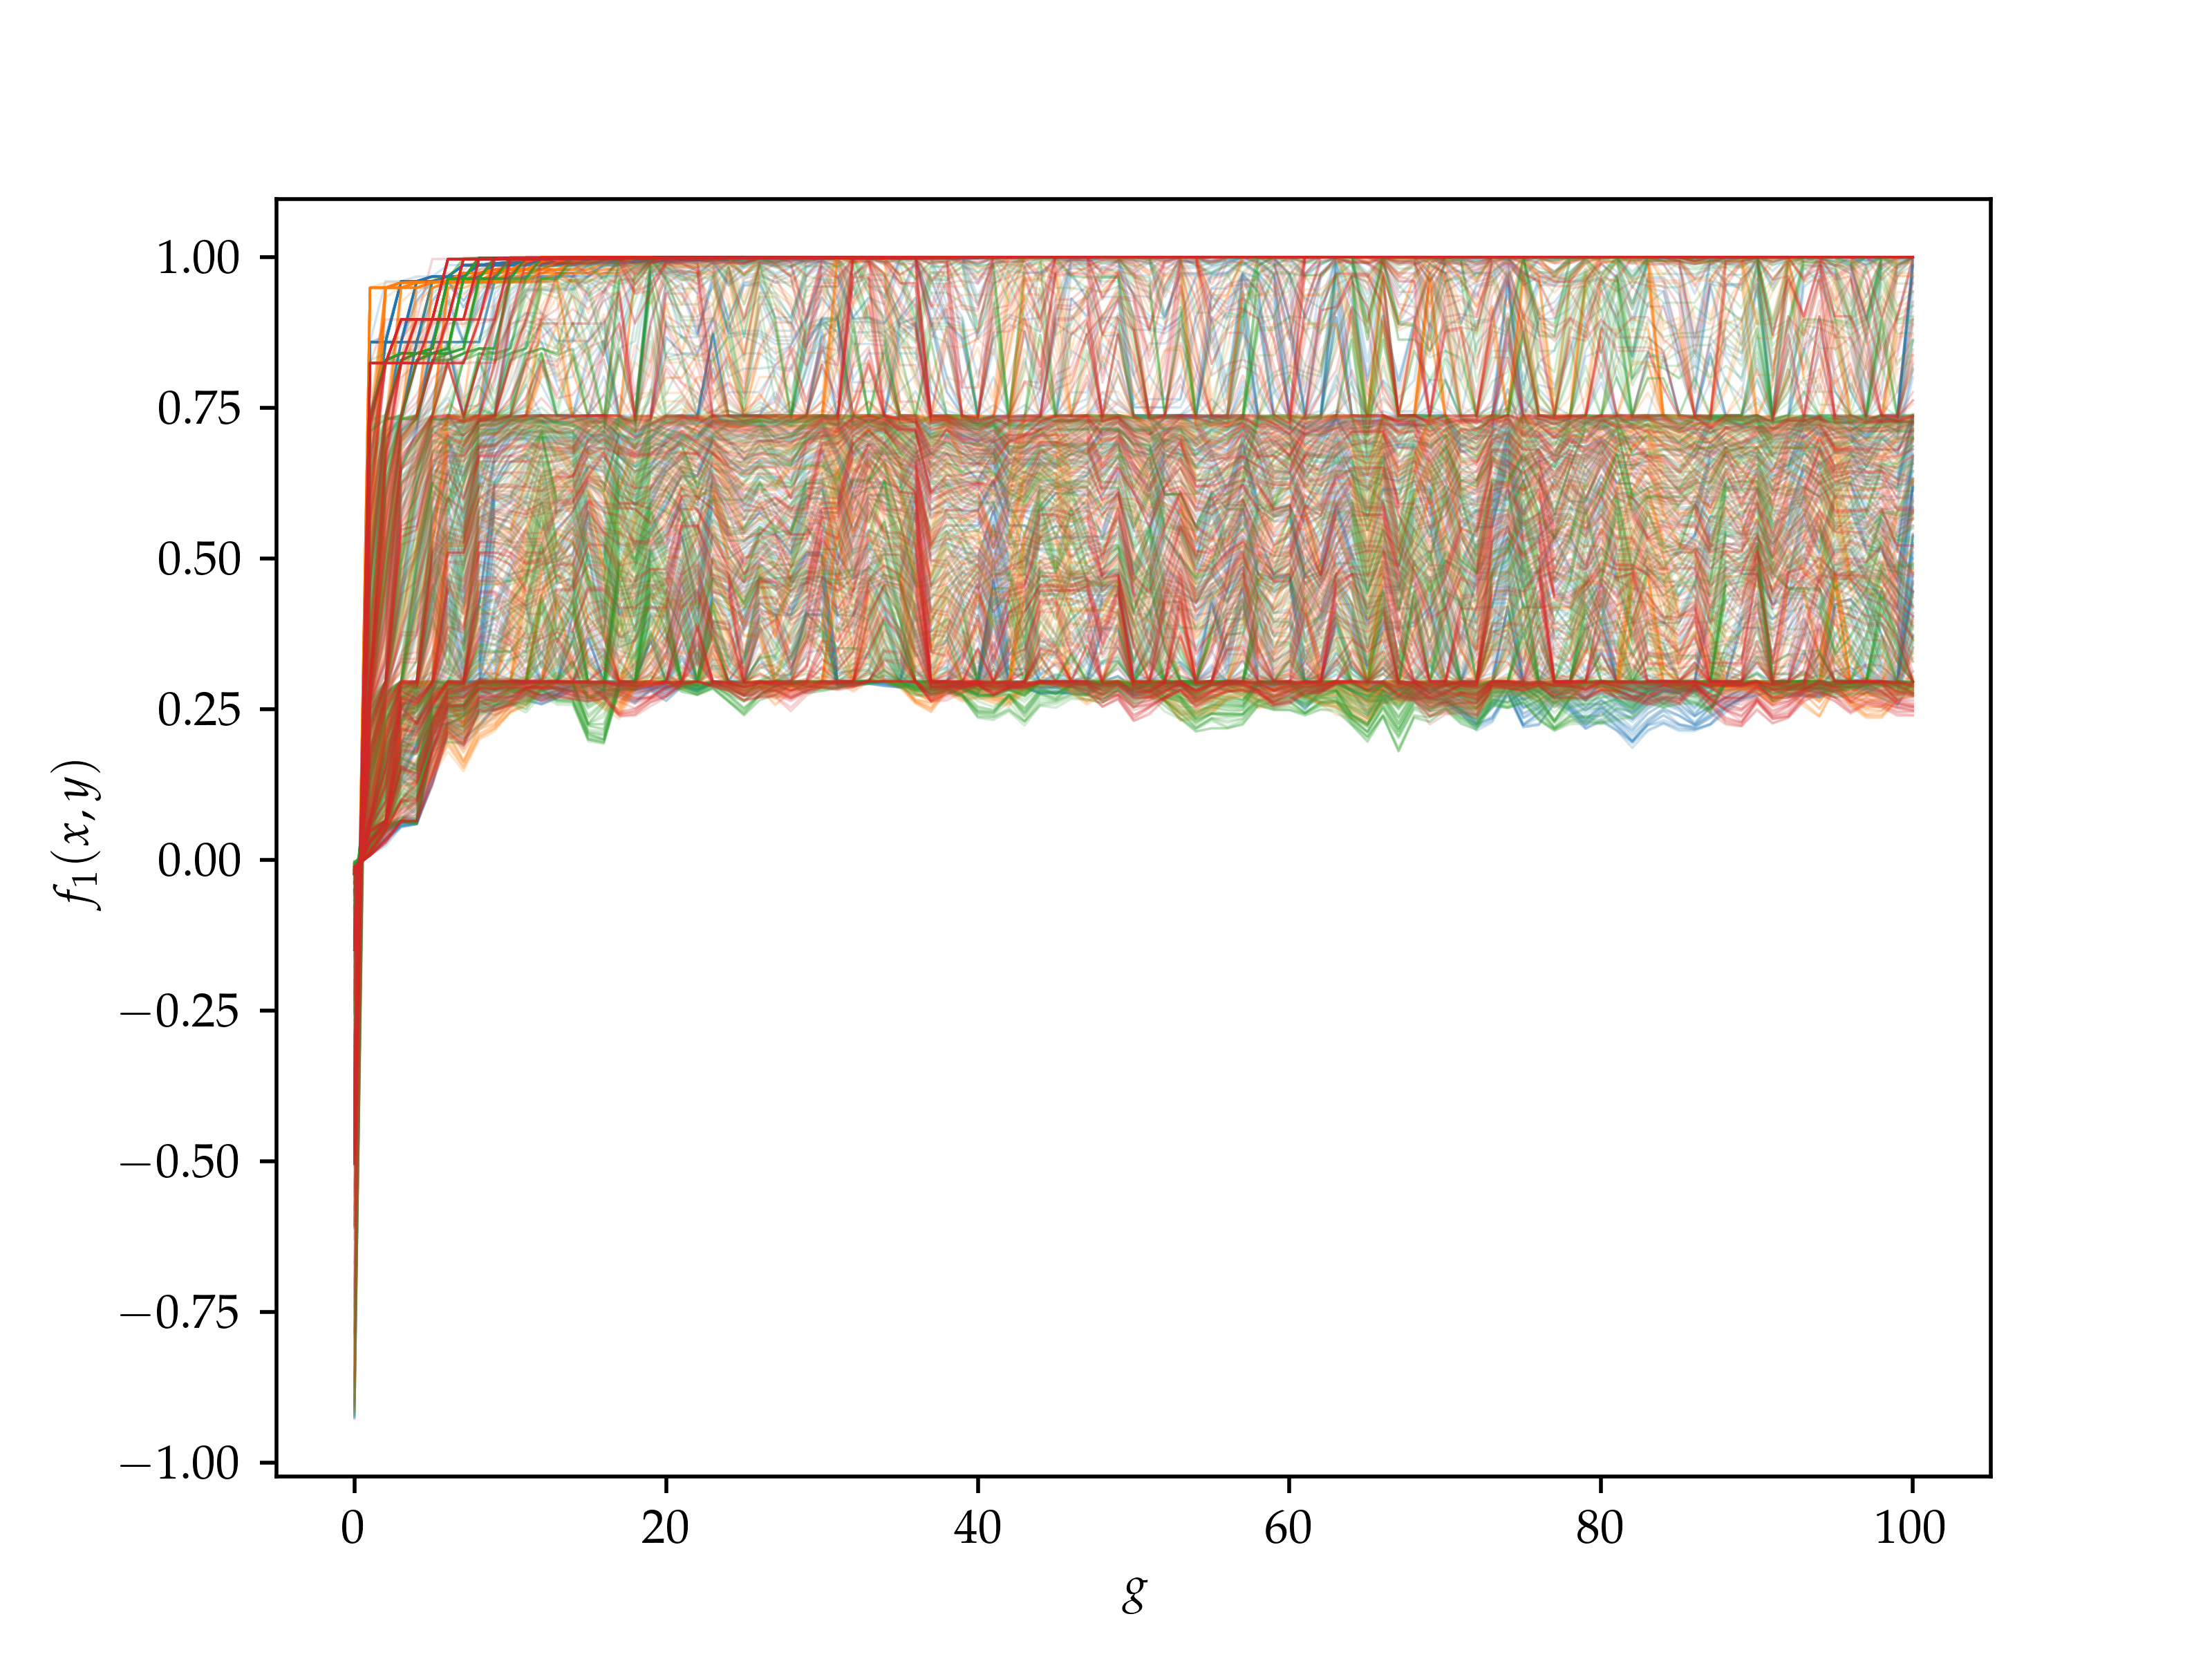
\includegraphics[width=\textwidth]{imagens/high_prob/evolution_damped_cossine.png}
  \caption{
    Evolução dos valores da função $ f_1(x,y) $ para os
    melhores 200 indivíduos de cada população, diferenciadas por cor, em termos da geração $g$,
    com $ p_2 = p_3 = 20\% $.
  }
  \label{fig:evolution_damped_cossine_mut_20}
\end{figure}

\begin{figure}[p]
  \centering
  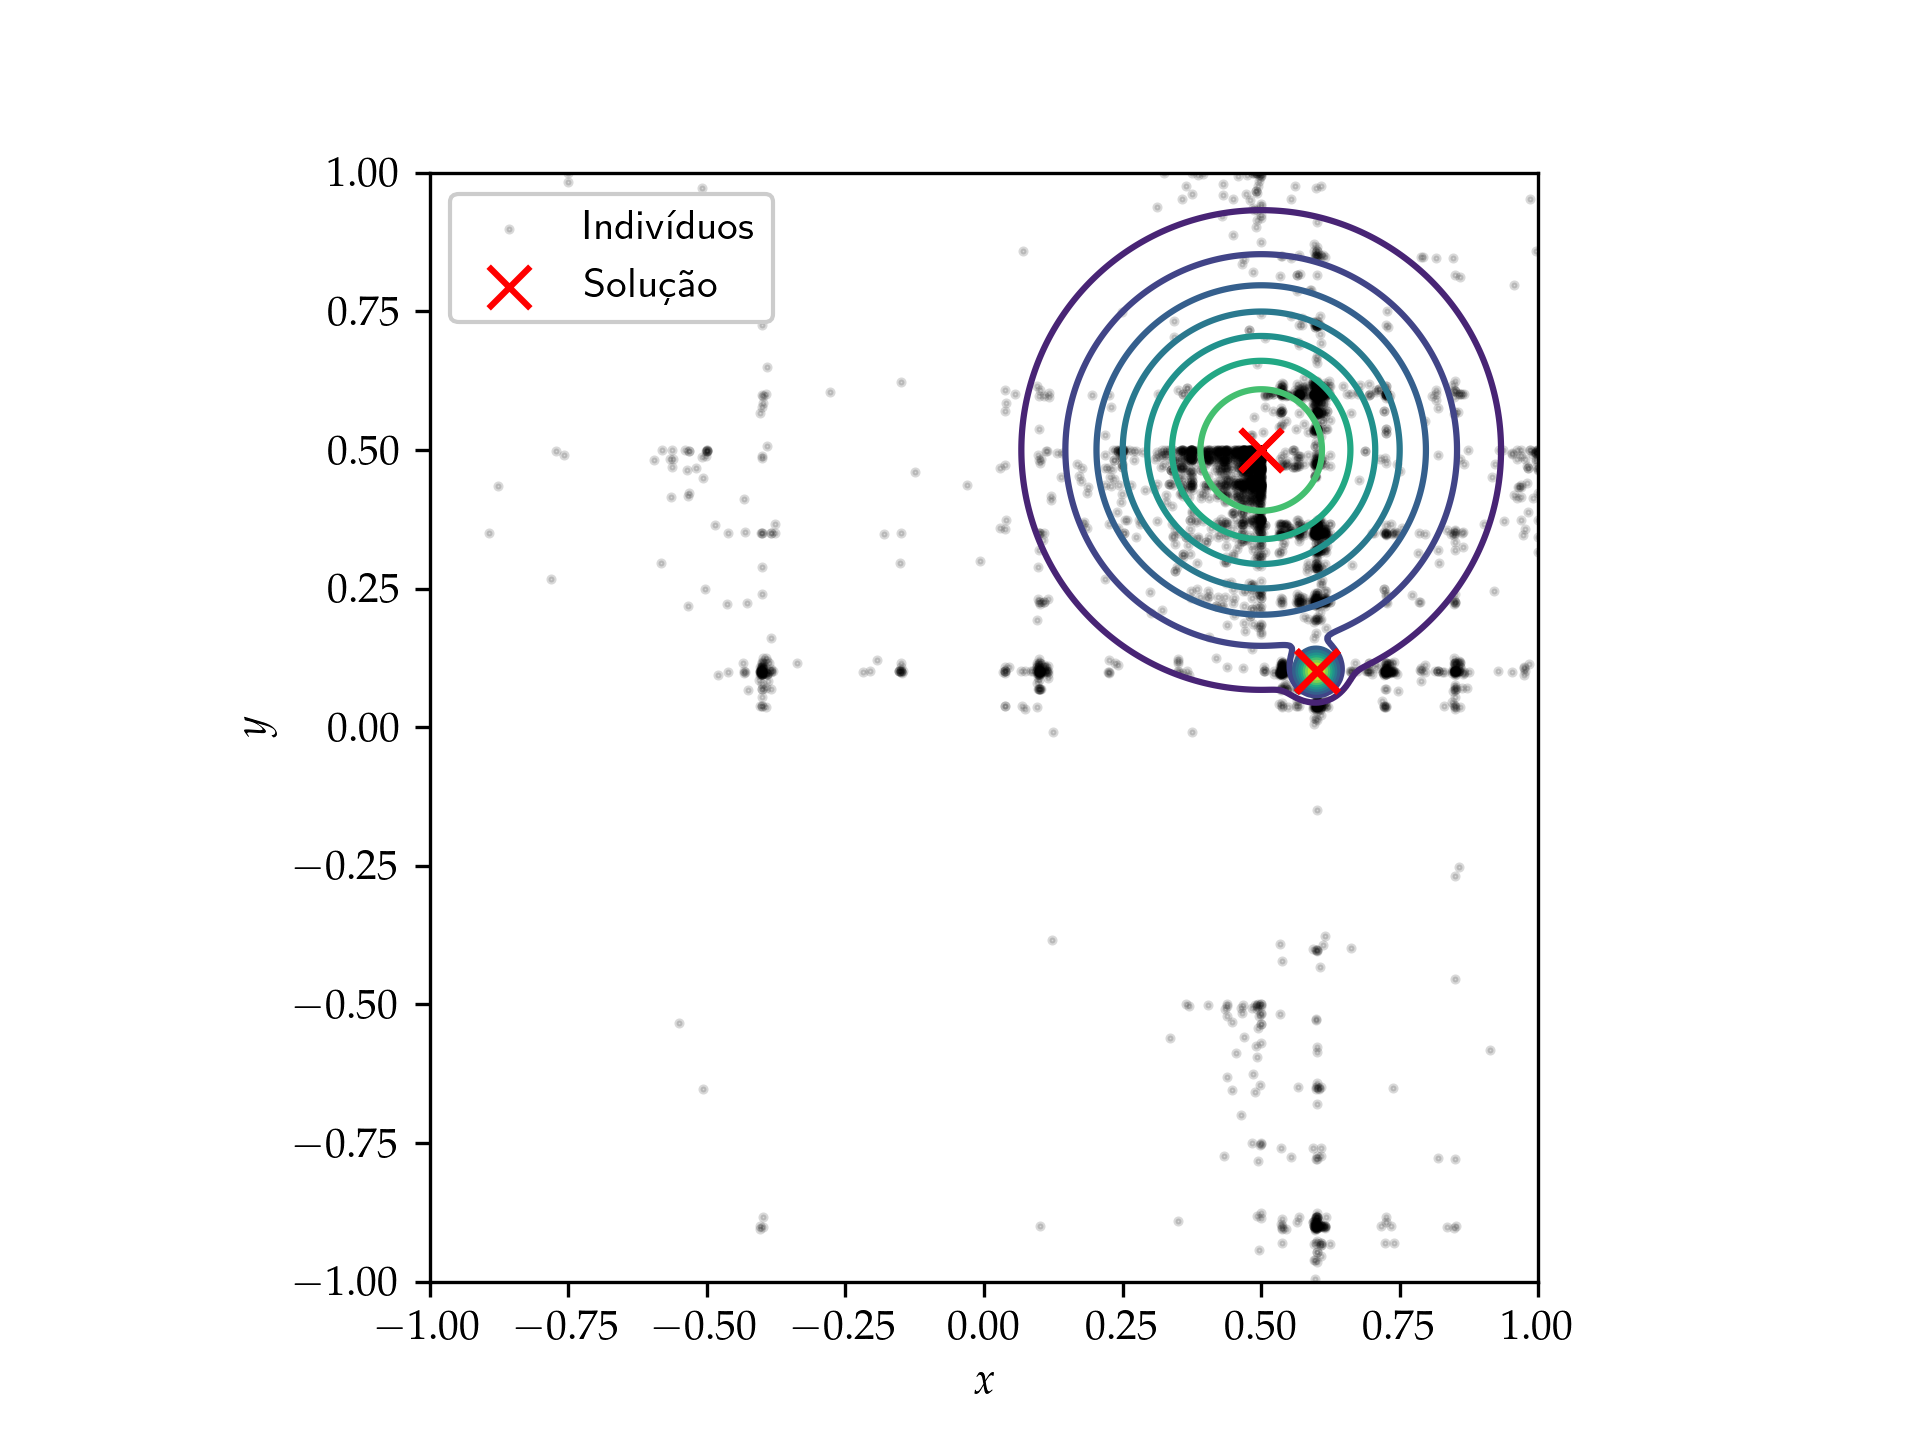
\includegraphics[width=\textwidth]{imagens/low_prob/contour_near_gaussians.png}
  \caption{
    Curvas de nível da função $f_2(x,y)$. Os pontos em preto indicam as posições dos indivíduos
    de 8 populações em sua 100ª geração na otimização da função, com $ p_2 = p_3 = 5\% $. 
    Marcado com um $\times$ vermelho estão os melhores indivíduos de cada população.
  }
  \label{fig:contour_near_gaussians}
\end{figure}

\begin{figure}[p]
  \centering
  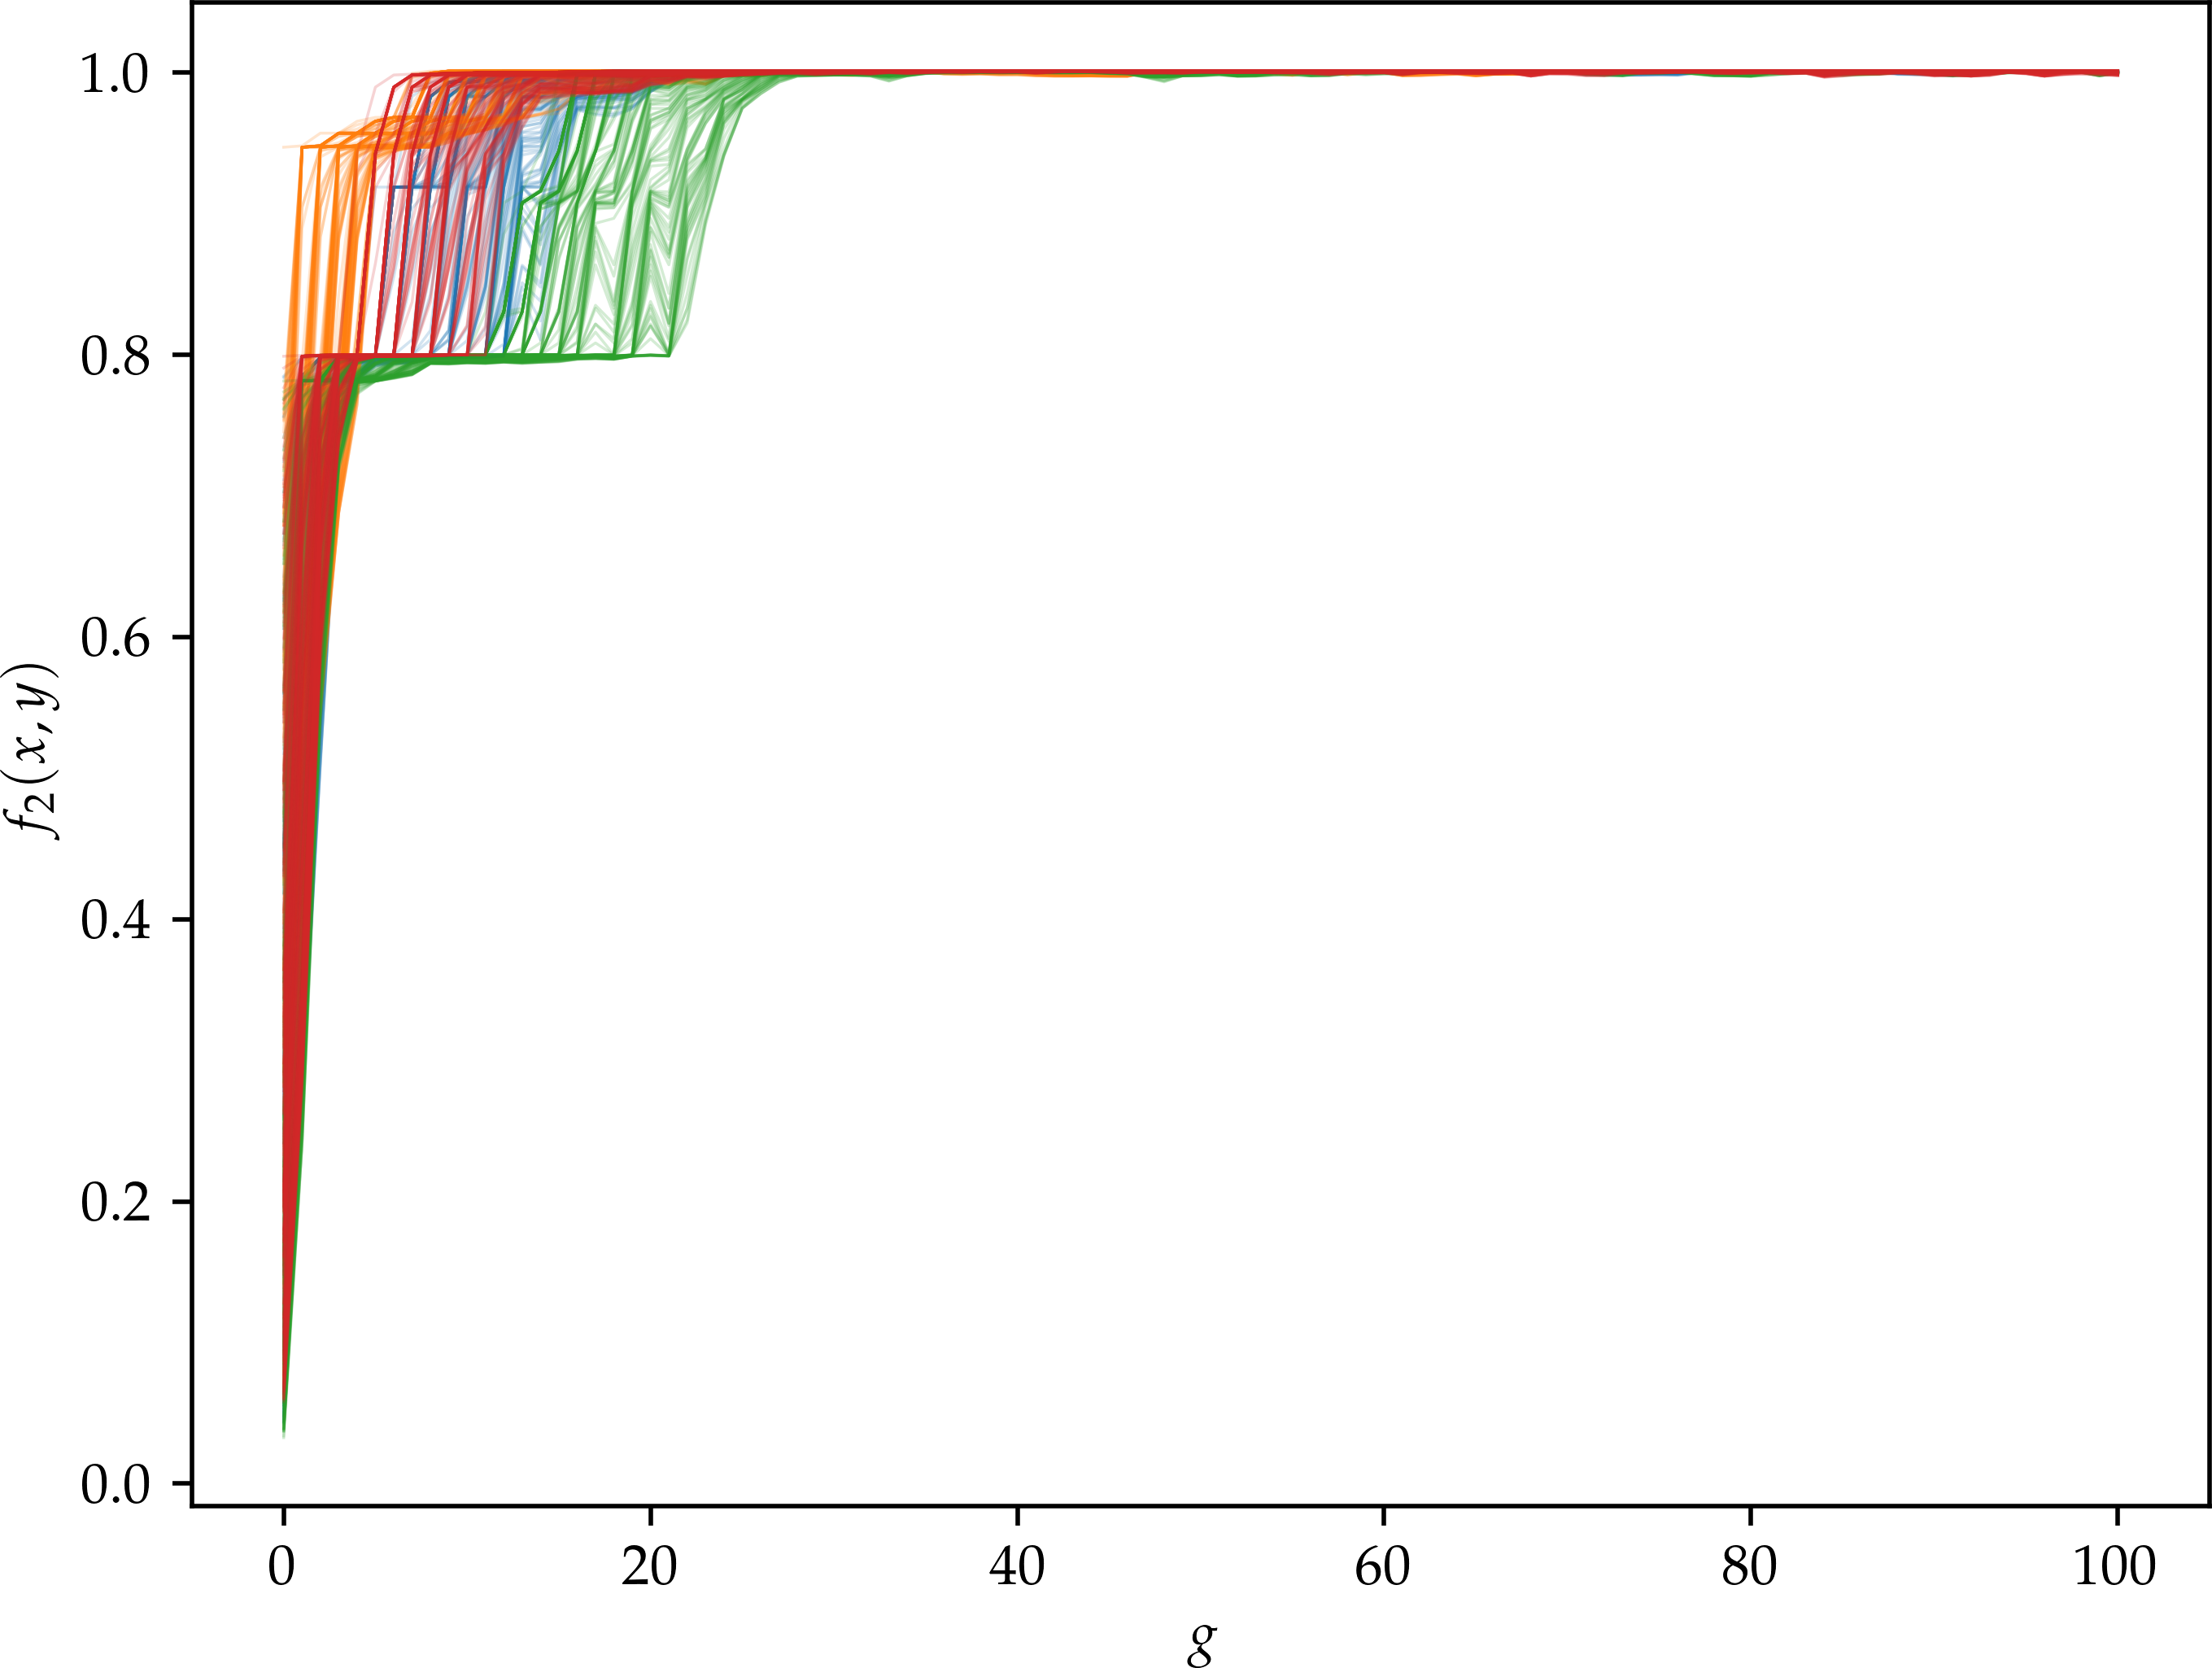
\includegraphics[width=\textwidth]{imagens/low_prob/evolution_near_gaussians.png}
  \caption{
    Evolução dos valores da função $ f_2(x,y) $ para os
    melhores 200 indivíduos de cada população, diferenciadas por cor, em termos da geração $g$,
    com $ p_2 = p_3 = 5\% $.
  }
  \label{fig:evolution_near_gaussians}
\end{figure}

\begin{figure}[p]
  \centering
  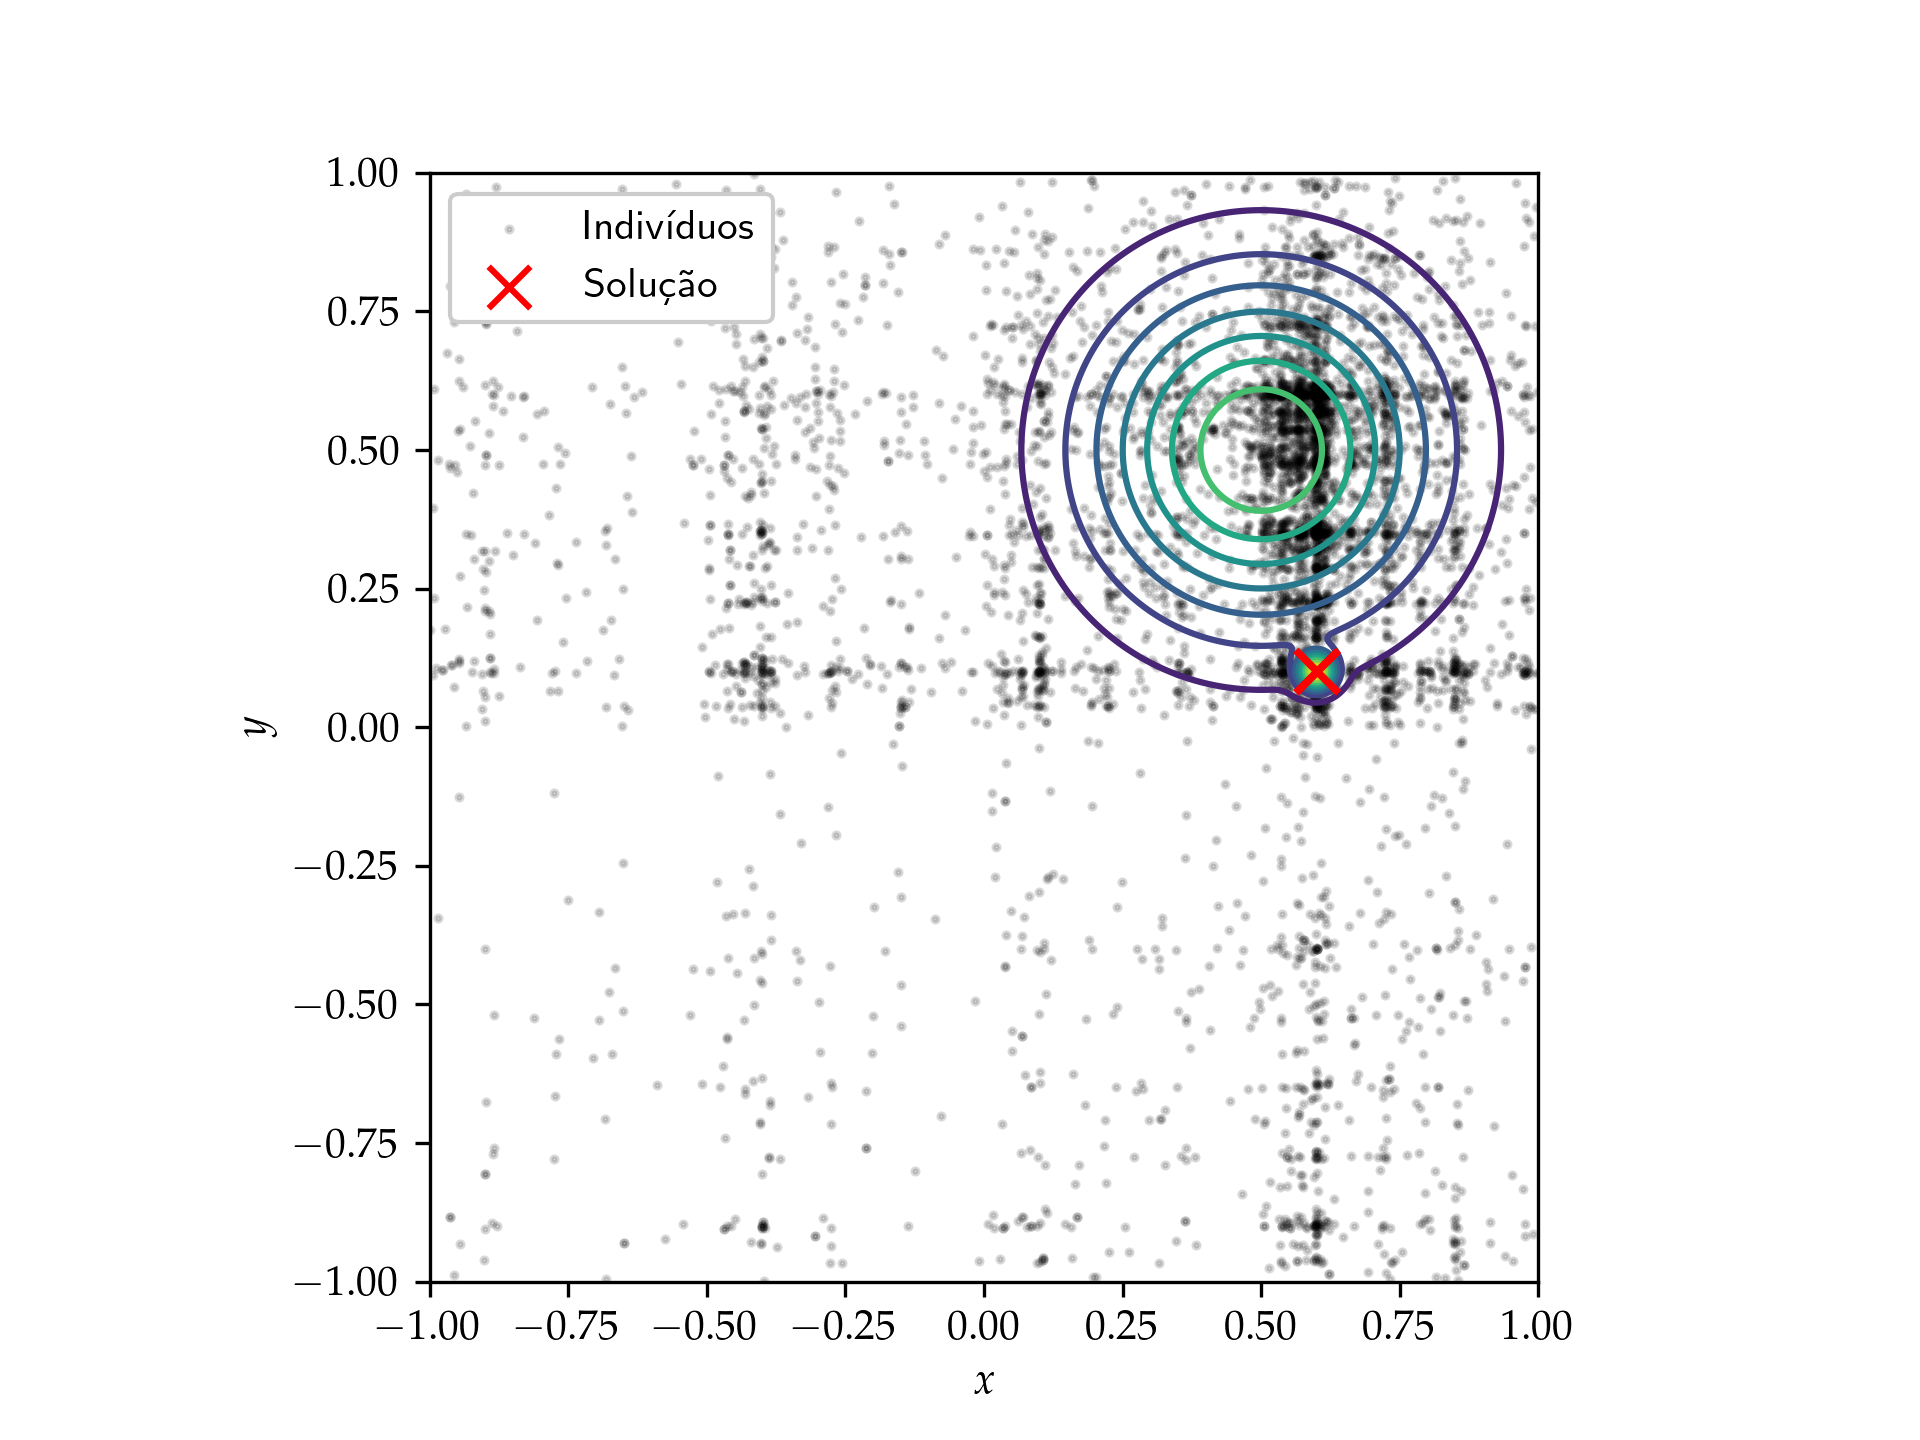
\includegraphics[width=\textwidth]{imagens/high_prob/contour_near_gaussians.png}
  \caption{
    Curvas de nível da função $f_2(x,y)$. Os pontos em preto indicam as posições dos indivíduos
    de 8 populações em sua 100ª geração na otimização da função, com $ p_2 = p_3 = 20\% $. 
    Marcado com um $\times$ vermelho estão os melhores indivíduos de cada população.
  }
  \label{fig:contour_near_gaussians_mut_20}
\end{figure}

\begin{figure}[p]
  \centering
  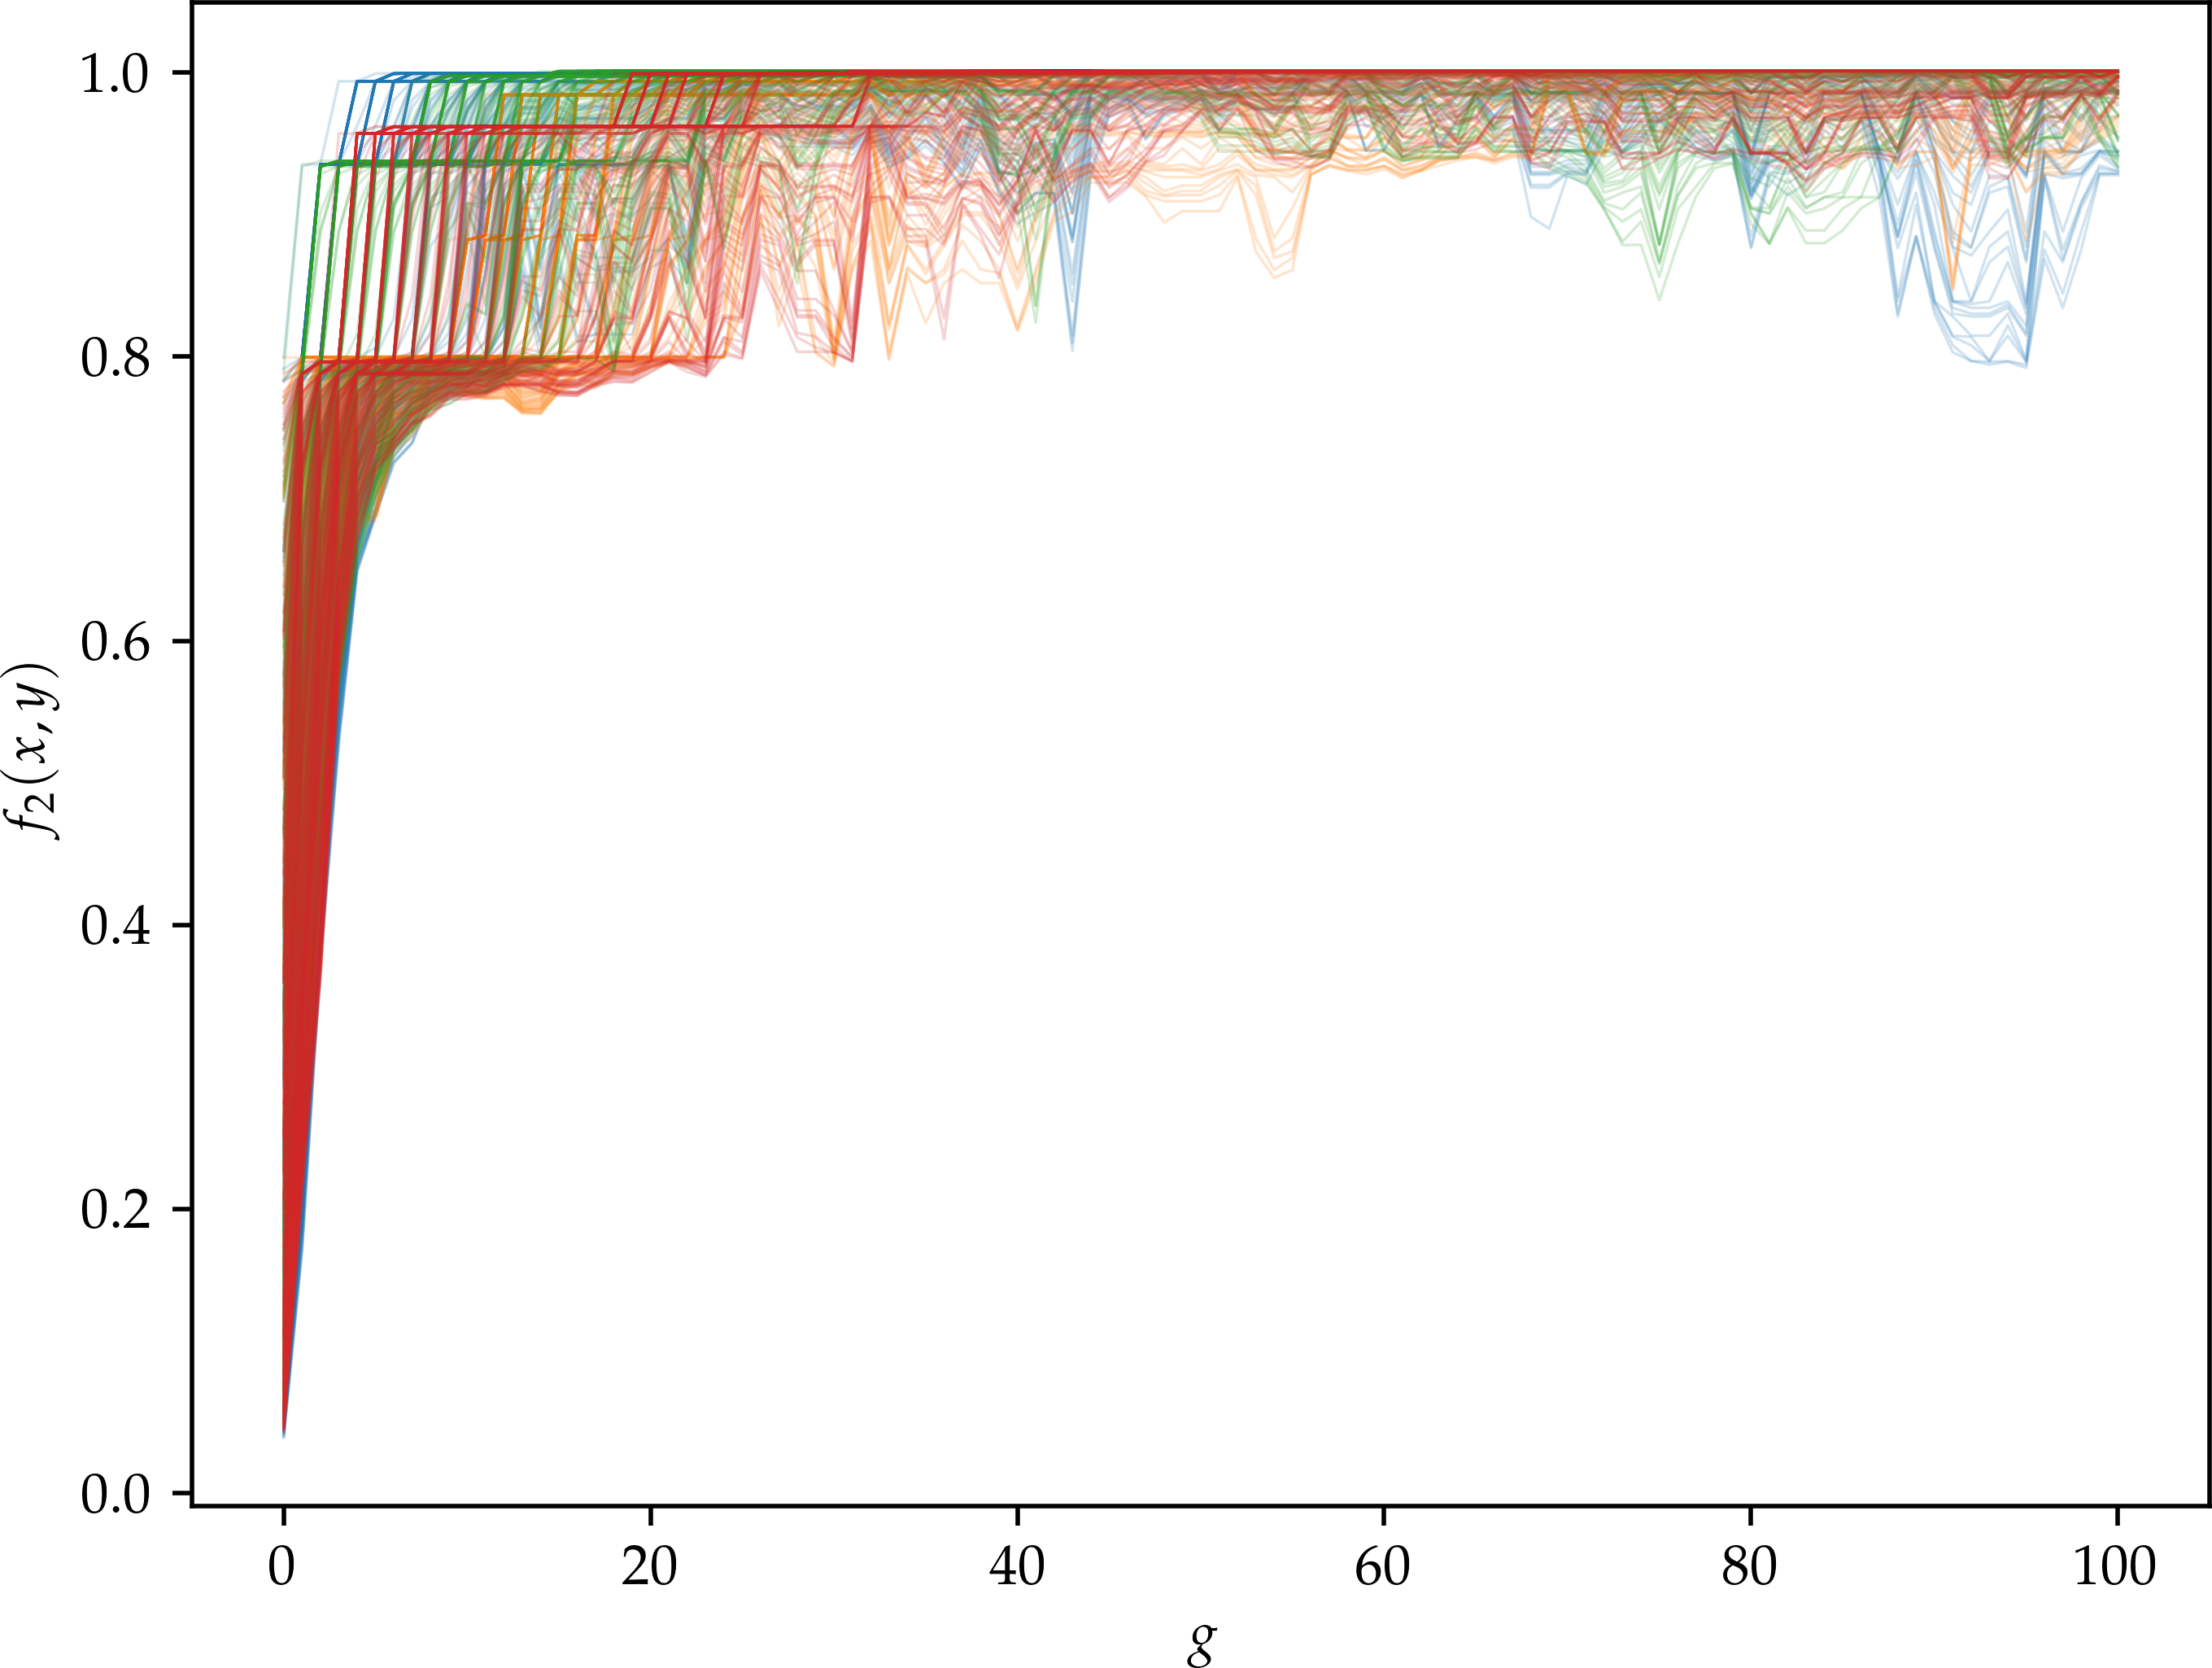
\includegraphics[width=\textwidth]{imagens/high_prob/evolution_near_gaussians.png}
  \caption{
    Evolução dos valores da função $ f_2(x,y) $ para os
    melhores 200 indivíduos de cada população, diferenciadas por cor, em termos da geração $g$,
    com $ p_2 = p_3 = 20\% $.
  }
  \label{fig:evolution_near_gaussians_mut_20}
\end{figure}

\section{Testes de Performance}

Em testes de tempo de execução o programa escalou bem, sendo sua complexidade temporal $\mathcal{O}(n)$ para o
tamanho de população, e $\mathcal{O}(g)$ para número de gerações decorridas. 
Nas figuras exibidas nesse capítulo, o tempo médio decorrido na evolução das populações de 1000 indivíduos
foi de 15 segundos\footnote{
  Tempo obtido usando uma máquina com processador Intel i7-8550U com frequência máxima de 4GHz.
  É importante frisar aqui as evoluções das 8 populações ocorreram em 8 processos em paralelo.
  Assim, é possível que, para uma única população, os tempos de execução sejam ligeiramente menores.
} enquanto que o tamanho da população necessário para que o processo tomasse mais de uma hora foi
superior a $n = 10^5$, para o mesmo número de gerações.

Isso mostra que a implementação é escalável para grandes valores de $n$, o que pode ser desejável em
algumas aplicações. É posto a prova também a performance da biblioteca NumPy, cujas funções e estruturas
de dados implementadas se mostraram altamente otimizadas.